% ===========================================================================
% fig-design-space.tex — router input design space: held-out cost saving by
% feature variant.
% BODY ONLY (tikzpicture). Wrapper/caption/label live in the section file.
% Requires % ===========================================================================
% fig-style.tex — shared colour / marker scheme for EVERY main-paper figure.
% \input this ONCE from the preamble of main.tex (after tikz + pgfplots).
%
% House rule: the palette is defined here and nowhere else. Each series also
% gets a distinct marker AND line style so the figures survive grayscale
% printing.
%
%   \sysname / deployed .. cSys   (blue!70!black)    mark *
%   opus / claude ........ cOpus  (red!70!black)     mark square*
%   gpt .................. cGpt   (teal!70!black)    mark triangle*
%   kimi ................. cKimi  (violet!70!black)  mark diamond*
%   flash ................ cFlash (orange!70!black)  mark pentagon*
%   greedy / baseline .... cBase  (gray)             mark o
% ===========================================================================
% The pipeline diagram needs the calc library for coordinate arithmetic; the
% rest of the libraries are already loaded in main.tex's preamble.
\usetikzlibrary{calc}
% Hatching, so bar charts stay readable in grayscale.
\usetikzlibrary{patterns}

\colorlet{cSys}{blue!70!black}
\colorlet{cOpus}{red!70!black}
\colorlet{cGpt}{teal!70!black}
\colorlet{cKimi}{violet!70!black}
\colorlet{cFlash}{orange!70!black}
\colorlet{cBase}{gray}

% Common axis furniture: footnotesize ticks/legend, small titles, framed
% legend in gray!50, light horizontal grid.
\pgfplotsset{
  paperaxis/.style={
    width=0.80\linewidth,
    height=5.2cm,
    tick label style={font=\footnotesize},
    label style={font=\footnotesize},
    title style={font=\small},
    legend style={font=\footnotesize, draw=gray!50, fill=white,
                  fill opacity=0.9, text opacity=1, rounded corners=1pt},
    every axis plot/.append style={line width=0.7pt},
    grid style={gray!25, line width=0.3pt},
    axis line style={gray!60},
    tick style={gray!60},
  },
  papermark/.style={mark size=2.6pt},
}
 in the preamble.
%
% PROVENANCE — every number.
%   Primary source: internal records, the definitive 4-row comparison on the
%   combined deployable router, column "saving %" (all four rows at the SAME matched accuracy .606,
%   fold-held-out, N=99, anchor = always-best gpt at $0.406 / .606):
%     A  task text only                              +30.5%  ($0.2824/task)
%     B  task text + handoff text                    + 8.0%  ($0.3734/task)
%     C  task text + hidden states                   +34.3%  ($0.2668/task)
%     D  task text + handoff text + hidden states    + 9.4%  ($0.3677/task)
%   Cross-checked against the same source's head-ablation table (LR rows:
%   30.5 / 8.0 / 34.3 / 9.4 — identical). Variant C, the text+hidden-state
%   blend, is the router's head; variant A is the text-only comparison.
%   The "handoff-text features hurt cost routing" reading is the source's
%   own: "The handoff-text embedding is a bad blend partner: averaging it in
%   (variants B and D) drags the saving down to ~8-9% ... so more features is
%   not better, the right feature is."
%   Fold stability (context, not plotted): A 3/5, B 1/5, C 3/5, D 4/5 vs
%   anchor; variant C's ~4pp gain over A is explicitly "not bankable at
%   N=99".
% ===========================================================================
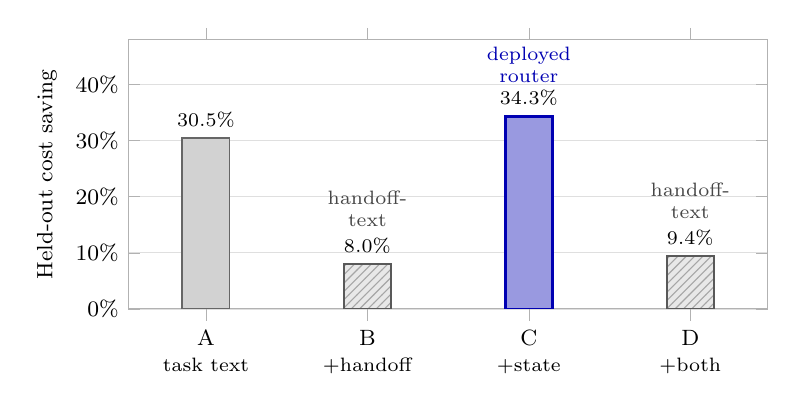
\begin{tikzpicture}
\begin{axis}[
  paperaxis,
  width=0.80\linewidth,
  height=5.0cm,
  ybar,
  bar width=17pt,
  ymin=0, ymax=48,
  ytick={0,10,20,30,40},
  yticklabel={\pgfmathprintnumber{\tick}\%},
  ylabel={Held-out cost saving},
  symbolic x coords={{A},{B},{C},{D}},
  xtick={{A},{B},{C},{D}},
  xticklabels={A\\{\scriptsize task text}, B\\{\scriptsize $+$handoff},
               C\\{\scriptsize $+$state}, D\\{\scriptsize $+$both}},
  xticklabel style={font=\footnotesize, align=center},
  enlarge x limits=0.16,
  ymajorgrids=true,
  nodes near coords={\pgfmathprintnumber[fixed, fixed zerofill, precision=1]{\pgfplotspointmeta}\%},
  nodes near coords style={font=\scriptsize},
]

% ---- A: text-only baseline --------------------------------------------
\addplot[fill=cBase!35, draw=cBase!80!black, bar shift=0pt]
  coordinates {({A},30.5)};

% ---- B and D: variants carrying handoff-text features (hatched) --------
\addplot[fill=cBase!18, draw=cBase!70!black, bar shift=0pt,
         postaction={pattern=north east lines, pattern color=cBase!70}]
  coordinates {({B},8.0) ({D},9.4)};

% ---- C: the winner, the deployed router --------------------------------
\addplot[fill=cSys!40, draw=cSys, line width=1.0pt, bar shift=0pt]
  coordinates {({C},34.3)};

% ---- winner callout ----------------------------------------------------
\node[font=\scriptsize, text=cSys, anchor=south, align=center]
  at (axis cs:{C},38.6) {deployed\\router};

% ---- the two handoff-text variants -------------------------------------
\node[font=\scriptsize, text=gray!55!black, anchor=south, align=center]
  at (axis cs:{B},13.0) {handoff-\\text};
\node[font=\scriptsize, text=gray!55!black, anchor=south, align=center]
  at (axis cs:{D},14.4) {handoff-\\text};

\end{axis}
\end{tikzpicture}
